\documentclass{CRPITStyle} 
\usepackage{harvard}  
\usepackage{graphicx}
\pagestyle{empty}
\thispagestyle{empty}
\hyphenation{roddick}
\bibliographystyle{agsm}   
\graphicspath{ {images/} }

\begin{document}

	\title {Software Development Life Cycles: History and Future}
	\author {Aden Kenny}
	\maketitle

	\begin {abstract} 
		This paper discusses the importance of the use of process models in the software development life cycle, provides a
		review of the process models used so far, compares and contrasts five different process models and then attempts to
		discuss the future of process models.
	\end {abstract}

	
	\section {Introduction} 
		\textit{The Software Crisis} was a time period in the infancy of software development where it was found to be difficult 
		to write software that was useful and efficient on the hardware of the time. This led to a large quantity of poor quality
		software being created that did not meet the requirements or was not even delivered at all.\\
		~\\
		It has been stated that there were problems of "achieving sufficient reliability" and difficulties of meeting time
		requirements and specifications on large scale projects amongst other problems that were discussed at the \textit{NATO
		Software Engineering Conference, 1968} (Naur and Randell, 1969).\\
		~\\
		As a result of this conference where major problems with the state of software development were brought up, software
		development process models started to become far more popular as they were seen as a major part of the solution to the
		\textit{Software Crisis}.

	\section {The importance of process models}
		During the \textit {Software Crisis} discussed above, many problems were faced possibly to the lack of direction in the
		development of software. These issues were things like projects being over budget, projects running over-time,
		inefficiency in the delivered software, projects that did not meet the set requirements, unmanageable projects, and
		projects that never delivered software. \\
		~\\
		 A solution that was proposed to the problems that software was facing was the idea
		of a development process guided by the usage of a framework. These frameworks later became known as 'process
		models'. \\
		~\\
		Nearly all software development process models start with a requirements gathering phase where the requirements that
		need to be met are gathered. This step is extremely important to the development of software as a program is highly
		unlikely to meet the requirements set by the client if the requirements have not been formally gathered and analysed.\\
		~\\
		A process model proves itself extremely useful in large scale, team projects. This is because a process model forms a 
		base on which a team can find a common understanding in the development of software. This is due to that idea that all
		software development projects have a process called the \textit{ software life cycle }. This involves a number of steps
		starting with "Requirements analysis and definition", "System design", "Program design", "Writing programs 
		(implementation)", "Testing", and "System delivery (deployment)" (Ma, 2017).\\
		~\\
		A set process model in a project means that a team will have a way of fulfilling the process of the software life cycle.
		This becomes important as it allows the team to have a common understanding what needs to be done at all times no
		matter what model is used. This common base of understanding, in theory, helps to mitigate some issues that both large scale
		and smaller scale software projects have faced in the past.\\
		~\\
		Large software projects are very complex and virtually all professional software developers and architects agree that the development
		of software requires analysis and synthesis (Ma, 2017). Analysis is the decomposition of a large scale problem into a smaller, more manageable
		pieces or a `divide and conquer' strategy. This requires abstracting problems from each other into independent sub-problems that have as
		few interdependencies as possible. These smaller sub-problems are then combined through Synthesis (Ma, 2017) which is the building (or composition) of
		a whole from smaller `building blocks'. In the case of software this is the composition of the sub-problems from the Analysis step. The composition stage
		is complex and can run into many issues.\\
		~\\
		Due to this complexity it is to have faults in the final software product and a way to address this issue is needed. The model development process
		helps to isolate locations in which certain kinds of faults are likely to manifest themselves. It additionally helps to find faults earlier and can help with
		building in fault tolerance.\\
		~\\
		A set, strict process allows a team to impose consistency and a set structure on a set of activities which leads to less faults in the process of the creation
		of software. A strong structure means that there is less freedom in the creation of software. This may sound like a negative idea but research and experience
		has shown a set process, even if it is a flexible process such as an agile method, will almost certainly deliver better results than an unstructured process 
		(Naur and Randell, 1969).\\
		
	\section {Review of proposed models}
	\subsection{Waterfall model}
		One of the first formally described process models was the the \textit{Waterfall model} by Winston Royce in 1970.
		Royce states that he believes in the concept of analysis before coding but presents the model as "risky" and that it
		"invites failure" (Royce, 1970).\\
		~\\
		One of the main ideas that can be taken away from Royce's paper is that analysis is a required step in the software development life cycle.
		This is very important as good software cannot be developed without fully understanding the problem that the software
		is designed to solve and all of the complexities involved, of which there will inevitably be many.\\
		~\\
		The waterfall model has been criticised as it is quite inflexible in some situations especially in the case of changing
		or unclear requirements. If a new requirement is requested or found to be needed it is not possible to go back a phase
		and insert this new requirement. The new requirement must either be ignored and not implemented, or the entire
		process must be restarted. Other problems include a long development time with nothing to show before the end and
		the idea that it "Views software development as [a] manufacturing process rather than a creative process" (Ma, 2017).\\
		~\\
		It was realised by some people quite soon after the adoption of the Waterfall method that it was flawed in some 
		situations such as by Royce where he first formally describes it and criticises it (Royce, 1970). This led to the
		development of other process models that were designed to fix the shortcomings of the waterfall model. Examples of
		these models include the ``Waterfall model with prototyping''. \\
		~\\
		 This is an arguably more flexible version of the Waterfall model. It involves following the same
		 design cycle as the waterfall model but involves prototyping in the design phase
		and the ability to move back to the requirements and system design phases in the testing phase.\\
		~\\
		The idea of a more flexible process model than waterfall has been frequently seen as advantageous in many situations
		which has recently led to more 'lightweight methods' gaining popularity. These lightweight methods generally focus 
		more on flexibility and the opportunity to go back to previous cycles to fix mistakes and add features that were not
		in the initial requirements, either through changing customer requirements or incomplete requirements gathering.\\
		~\\
		The Waterfall model has been described as a "heavyweight method" (Ma, 2017). These 'heavyweight methods' 
		do have advantages over so called 'lightweight models'. The waterfall model provides an extremely useful case
		to examine the advantages of heavyweight models as it is possibly the most frequently used heavyweight model
		and because of its long history and the large amount of use it has had. \\
		~\\
		One of the main cited advantages of the Waterfall model is it is frequently possible that errors in design are found
		before any code is actually written (Hughey, 2009). This saves time during the implementation phase as 
		there will be no need, in an ideal situation, to go back to the planning stage of the life cycle. An additional frequently
		mentioned advantage is the idea that a very structured model means that it is far easier to measure the progress of the project
		when compared to more lightweight models, as the project milestones are clearly defined.\\
		~\\
		\subsection{Scrum model}
		One major agile method is the `Scrum' model. Scrum is both iterative and incremental (Rising and Janoff, 2000), and is designed to be flexible towards changing
		customer requirements. The Scrum model calls for small teams that work together very closely. This requirement is due to research showing that small, interconnected teams perform better when developing software (Rising and Janoff, 2000). This closeness of team is manifested with daily `standups' which are whole team
		meetings where the project is discussed, future plans are considered and responsibilities are delegated out.\\
		~\\
		A key idea of the Scrum model is when developing a software project, the requirements are likely to be volatile and change due to changing requirements from
		the customer and that the changing requirements are better addressed with this agile, iterative approach when compared to more traditional heavyweight model such as Waterfall.\\
		~\\
		Scrum is commonly referred to as a ``feedback-driven empirical approach'', and this is clearly shown by the importance of customer feedback in the Scrum model. 
		In Scrum there are three main defined roles, these roles together make up the `Scrum Team'. Firstly is the `Product Owner', the Product Owner represents the
		customer and all stakeholders (Rising and Janoff, 2000) and should not be involved in the technical solution, the Product Owner should focus on the requirements
		and business aspects of the project. The next role is the ``Development Team'', the team is generally made up of 3 to 9 people (Rising and Janoff, 2000) who do
		the technical work on the project. This ranges from things such as requirements analysis to the actual development of the product to testing and documentation.
		The final defined role is the `Scrum Master', this person ``leads the Scrum meetings, identifies the initial backlog to be completed in the sprint, and empirically measures progress toward the goal of delivering this incremental set of product functionality.  The Scrum master ensures that everyone makes progress, records the decisions made at the meeting and tracks action items, and keeps the Scrum meetings short and focused'' (Rising and Janoff, 2000). Therefore the Scrum master can be thought of as a project leader or manager.\\
		~\\
		\subsection{Extreme Programming}
		The other agile method discussed will be `Extreme Programming'. Extreme Programming``is a lightweight methodology based on addressing constraints in software development'' (Ma, 2017).  A major strength of Extreme Programming is its ability to adapt to vague or rapidly changing requirements. This is due to the central principles of Extreme Programming which include `Rapid
		feedback' which means that the development team gets frequent feedback from the customers which allows for flexiblity in the project as a whole. This ``feedback
		allows the team to adapt rapidly to changing requirements which seem to be more and more frequent in the modern development environment''.\\
		~\\
		Extreme Programming is named due to the idea that it takes the best practices of traditional software development and takes them to extreme levels. For example
		peer reviewing of code is generally considered to be good practice and Extreme Programming can take this to the extreme with `pair programming' where two programmers code at one computer with one person writing the code and the other person acting as a sort of `navigator'. The navigator controls the strategy of the work and the overall picture which allows the person coding to focus on the technical challenges of the current task.\\
		~\\
		Extreme Programming also takes customer feedback to the extreme. This is done through often having a representative for the customer on site while the software
		is being developed. This means that customer feedback can very quickly and very frequently be sought allowing for changes to be picked up quickly and worked on.
		The idea of an on site customer in Extreme Programming stems from the idea that it is almost impossible to fully understand a customers requirements for a large
		scale software project therefore constant feedback and frequent iterations are needed in order to fufill the needs and requirements of the customers towards the project.
		
		\subsection{V model}~\\
		\\
		The V model can be considered an extension of the Waterfall model but instead of a linear progression towards the delivery of a product, the V model
		
		\begin{figure}
		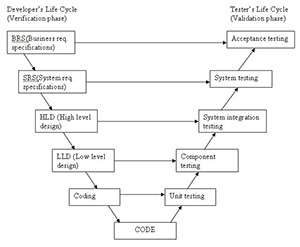
\includegraphics{VModel1}
		~\\
		\caption{\protect\label{VModel} A diagram of the V model (V model diagram, n.d).}
		\end{figure}
		
	\section {Comparison of process models}
	
		This section will compare and contrast five different process models.\\
		~\\
		These models are as follows:
		~\\
		\begin{itemize}
			\item Waterfall model
			\item Spiral model
			\item V model
			\item Extreme Programming
			\item Scrum
		\end{itemize}~\\
		
		In order to simplify discussion of these five models they will broken down into three different groups. First we have the so called `lightweight
		methods' which consists of Extreme Programming and Scrum. Secondly we have the more `heavyweight methods' which consists of Waterfall and the V model. Finally
		we have the Spiral model which does not quite fit into either category. It has many similarities to the heavyweights such as a similar life cycle, but
		done multiple times, as required, and similarities to the lightweights such as multiple iterations (which is the life cycle done multiple times). It also
		has unique features which the heavyweights and the lightweights do not have such as a strong focus on risk management. We will place the
		Spiral into its own category of `intermediate methods'.\\
		~\\
		First to be discussed will be the Waterfall model. As previously mentioned in above sections the waterfall model has been criticised
		but still remains one of the most used process models.
		This is because while it has some disadvantages it also has a significant amount of advantages (Ma, 2017) along with a long history of usage.\\
		~\\
		\begin{figure}
		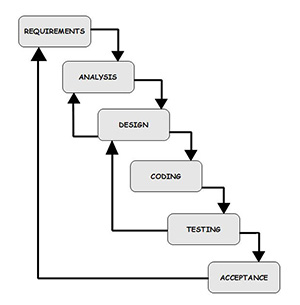
\includegraphics{waterfall2}
		~\\
		\caption{\protect\label{waterfall} A diagram of the Waterfall model (Waterfall model diagram, n.d).}
		\end{figure}
		It ``works for well understood problems with minimal or no changes in the requirements'' (Ma, 2017). This is due to the fact that
		it does not provide for iterative development so all work that is done works towards the set requirements, and if the requirements
		that are set at the start of the project remain constant it allows for potentially faster delivery when compared to a more lightweight
		model such as Scrum which calls for a more flexible approach based around the idea that a problem cannot be fully defined, so it focuses
		more on quick iterations based around changing requirements.\\
		~\\
		Waterfall, along with the V model that it is the parent of, are the only two models discussed here that do not provide for iterative
		development. Extreme Programming and Scrum provide for it as they are Agile methodologies and Agile calls for iterative development.\\
		~\\
		 The other model that will be discussed is the Spiral model. The Spiral model was first introduced by Barry Boehm in 
		 1986 as a ``candidate for improving the software process model situation'' (Boehm, 1986). It is stated that it creates a ``risk-driven
		 approach to the software process' (Boehm, 1986).\\
		 ~\\
		 
		 \begin{figure}
		  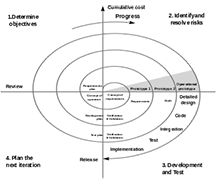
\includegraphics{spiral1}\\
		  ~\\
		  \caption{\protect\label{spiral} A diagram of the Spiral model (Boehm, 1988).}
		  \end{figure}
		The Spiral calls for multiple iterations like the lightweights but each of these iterations being so called `cycles', and each Waterfall
		activity becomes a cycle. The Spiral does differ from the lightweights as ``The Spiral model can deal with change between phases, but does not allow change within a phase (Ma, 2017)''. This is also in contrast to Waterfall which, when a phase is completed does not allow going back and reopening new issues that have arisen. This makes the Spiral model arguably more flexible in regards to mistakes and changing requirements when compared to the Waterfall model.\\
		~\\
		Due to the fact that the Spiral model does not allow change within a phase there is a need for a model if change is happening very quite frequently. These models are the lightweight, Agile models. All Agile models call for the ability to deal with rapid changes in requirements. This, in the case of the Scrum and Extreme Programming models, is done through rapid iterations generally ranging from around one to four weeks. \\
		~\\
		In the case of Extreme Programming, these rapid iterations involve constant client feedback, frequently with an on site client. At the end of an iteration the resulting product is shown to the customer and feedback is sought. This leads to feedback that will be useful in the next iteration. The Scrum process is fairly similar but an iteration is generally called a `sprint'. Once a sprint has finished ``all project teams meet with all stakeholders ... At this meeting \textit{anything} can be changed'' (Rising and Janoff, 2000). This is obviously quite similar to Extreme Programming but Scrum does not generally call for an on site client. This is in direct contrast to the heavyweight methods which do not have frequent customer feedback involved.\\
		~\\
				A major difference between the heavyweight and lightweight methodologies that it is frequently cited is the idea of iterative development. More 
		lightweight, agile, methods such as Scrum or Extreme Programming require that features are developed iteratively
		and favours short release cycles with frequent feedback from the customer. This is contrast to so called 'less flexible'
		models like waterfall. These more heavyweight models call for a single release at the end. Critics of waterfall state
		that this can be harmful to the project as it becomes extremely infeasible to get customer or stakeholder feedback
		on the current state of the project.\\
		~\\

\begin{thebibliography}{xx}

	\harvarditem{[Naur and Randell]}
  	{1969}{null}
	Naur, P. \harvardand\ Randell, B.  \harvardyearleft
  	1969\harvardyearright , "Software Engineering - Report on a conference sponsored by the NATO Science Committee".
	
	\harvarditem{[Royce]}
	{1970}{null}
	Royce, W. \harvardyearleft
	1970\harvardyearright, "Managing the Development of Large Software Systems," {\em in} Proceedings of IEEE WESCON.

	\harvarditem{[Ma]}
	{2017}{null}
	Ma, H. \harvardyearleft
	2017\harvardyearright, "Classical Software Life Cycle Models" from lecture notes distributed in SWEN301.
	
	\harvarditem{[Larman]}
	{2003}{null}
	Larman, C. \harvardand\ Basili, V. \harvardyearleft
	2003\harvardyearright, "Iterative and Incremental Development: A Brief History,"\textit{ IEEE Computer,} vol. 36, pp. 47-56, June 2003.
	
	\harvarditem{[Hughey]}
	{2009}{null}
	Hughey, D. \harvardyearleft
	2009\harvardyearright, "Comparing Traditional Systems Analysis and Design with Agile Methodologies". University of
	Missouri - St. Louis.
	
	\harvarditem{[Boehm]}
	{1986}{null}
	Bohem, B. \harvardyearleft
	1986\harvardyearright, ``A Spiral Model of Software Development and Enhancement,''\textit{ ACM SIGSOFT Software Engineering
	Notes}, vol. 11, no. 4, pp. 14 - 24, August 1986.
	
	\harvarditem{[Bassil]}
	{2012}{null}
	Bassil, Y. \harvardyearleft
	2012\harvardyearright, ``A Simulation Model for the Waterfall Software Development Life Cycle,'' \textit{International Journal of Engineering \&\ Technology},
	vol. 2, No. 5, May 2012.
	
	\harvarditem{[Rising]}
	{2000}{null}
	Rising, L. \harvardand\ Janoff, N.S. \harvardyearleft
	2000\harvardyearright, ``The Scrum software development process for small teams,''\textit{ IEEE Software}, vol. 17, no. 4, pp. 26 - 32, July/August 2000. 
	
	\harvarditem{[Mahanti]}
	{2012}{null}
	Mahanti, R., Neogi, M.S. \harvardand\ Bhattacherjee, V. \harvardyearleft
	2012\harvardyearright, ``Factors Affecting the Choice of Software Life Cycle Models in the Software Industry - An Empirical Study,''\textit{Journal of Computer Science},
	vol. 8, no. 8, pp. 1253 - 1262, 2012.
	
	\harvarditem{[Boehm2]}
	{1988}{null}
	Boehm, B. \harvardyearleft
	1988\harvardyearright, \textit{Spiral model}, diagram, viewed April 2017,
	https://upload.wikimedia.org/wikipedia/commons
/thumb/e/ec/Spiral\_model\_\%28Boehm\%2C\_1988
	\%29.svg/333px-Spiral\_model\_\%28Boehm
	\%2C\_1988\%29.svg.png/
	
	\harvarditem{[Sharma]}
	{2016}{null}
	Sharma, P. \harvardand\ Hasteer, N. \harvardyearleft
	2016\harvardyearright, ``Analysis of linear sequential and extreme programming development methodology for a gaming application,'' \textit{ Communication and Signal Processing (ICCSP), 2016 International Conference on}, April 2016.
	
	\harvarditem{[WaterfallDiagram]}
	{n.d}{null}
	\textit{Waterfall model diagram,} n.d. diagram, viewed 7 April 2017, http://www.buzzle.com/images/diagrams/waterfall-model-diagram.jpg.
	
	\harvarditem{[VModelDiagram]}
	{n.d}{null}
	\textit{V model diagram,} n.d. diagram, viewed 7 April 2017, http://istqbexamcertification.com/wp-content/uploads/2012/01/V-model.jpg.
	
	\harvarditem{[agileManifesto]}
	{2001}{null}
	Beck, K., Beedle, M., van Bennekum, A., Cockburn, A., Cunningham, W., Fowler, M., Grenning, J., Highsmith, J., Hunt, A., Jeffries, R., Kern, J., Marick, B., Martin, R.C,
	Mellor, S., Schwaber, K., Sutherland, J. \harvardand\ Thomas, D. \harvardyearleft
	2001\harvardyearright, \textit{Manifesto for Agile Software Development}, viewed 5 April 2017, http://agilemanifesto.org/.
	
\end{thebibliography}
		

\end{document}